% Pacotes e configurações padrão do estilo "article"\
% -------------------------------------
\documentclass[a4paper,12pt]{article}
% Layout
% --------------------------------------------------------------------------------
\usepackage{pdfpages} % Pacote para inserir um PDF dentro do LaTeX
\usepackage{minted} % Pacote para Colorir Código
\usepackage{circuitikz}
\usepackage{verbatim}
\usepackage[portuges]{babel}
%     Gráficos e layout ----------------------------------------------------------------------
\ifx\pdfmatch\undefined
\else
    \usepackage[T1]{fontenc}
    \usepackage[utf8]{inputenc}
\fi
% xetex:
\ifx\XeTeXinterchartoks\undefined
\else
    \usepackage{fontspec}
    \defaultfontfeatures{Ligatures=TeX}
\fi
% luatex:
\ifx\directlua\undefined
\else
    \usepackage{fontspec}
\fi
% End engine-specific settings

%      Fonte --------------------------------------------------------------------------------
%\usepackage{lmodern}
\usepackage{times}
%     Pacotes adicionados -------------------------------------------------------------------
\usepackage{ae}
%     Língua e hifenização ------------------------------------------------------------------
\usepackage[english]{babel}
\usepackage{hyphenat}
% ---------------------------------------------------------------------------------------
\usepackage{fancyhdr}
\usepackage{sectsty}
\usepackage{float}
%\usepackage{graphicx}
%\usepackage[pdftex]{color,graphicx}
\usepackage{hyperref}
\usepackage{enumerate} % Permite alterar Layout do enumerate
%\usepackage{pdflscape} % Permite alterar a orientação da pagina
%\usepackage{ifthen} % Permite usar condicionais ifelse
%\usepackage[table]{xcolor} % Permite alterar as cores das celulas de uma tabela
\usepackage{amsmath,amssymb} % Ambiente para uso de elementos matemáticos
\usepackage{caption}
\usepackage{subcaption} % permite o uso de multiplas figuras com legenda
%     Dados do título e autores --------------------------------------------------------------
%\title{\tituloRelatorio}
\author{Rafael Lima}
%     Definições do pdf ----------------------------------------------------------------------
\hypersetup{
    unicode=false,          % non-Latin characters in Acrobat’s bookmarks
    pdftoolbar=true,        % show Acrobat’s toolbar?
    pdfmenubar=true,        % show Acrobat’s menu?
    pdffitwindow=false,     % window fit to page when opened
    pdfstartview={FitH},    % fits the width of the page to the window    
    pdfauthor={Rafael Lima},     % author
    pdfnewwindow=true      % links in new window
}
% Layout do documento ------------------------------------------------------------------------
 \pagestyle{fancy}
%     Cabeçalho e Rodapé ---------------------------------------------------------------
      \lhead{}
      \chead{}
      \rhead{}
      \lfoot{}
      \cfoot{}
      \rfoot{\thepage}
      %     Númeração ------------------------------------------------------------------------
      \pagenumbering{arabic}
      %     Retas do cabeçalho e rodapé ------------------------------------------------------
      \renewcommand{\headrulewidth}{0.5pt}
      \renewcommand{\footrulewidth}{0.5pt}
      %     Tamanho da letra de seções e derivadas --------------------------------------------
      \sectionfont{\normalsize}
      \subsectionfont{\small}
      %     Hiperlinks ------------------------------------------------------------------------
      \hypersetup{
                  colorlinks,
                  citecolor=black,
                  filecolor=black,
                  linkcolor=black,
                  urlcolor=black
                  }
%     Outros ----------------------------------------------------------------------------
      \addto\captionsbrazilian{\renewcommand{\contentsname}{Índice}} % Muda nome dos contents
      %\renewcommand{\thesection}{(\alph{section})} % muda o estilo de númeração das sections
      % alterando a formatação dos numeradores de lista de itens
      \renewcommand\theenumi{\arabic{enumi}}
      \renewcommand\labelenumi{(\textit{\theenumi})}
	  \renewcommand\theenumii{\arabic{enumii}}
	  \renewcommand\labelenumii{(\textit{\theenumi.\theenumii})}
      
% ---------------------------------------------------------------------------------------

\newcommand{\tituloRelatorio}{Jornal Entry - Class 1}
\title{\tituloRelatorio}
\hypersetup{pdftitle={\tituloRelatorio}}% title

\usepackage{listings}
\lstset{
  language=Matlab,
  basicstyle=\ttfamily\small, 
  keywordstyle=\color{blue}, 
  stringstyle=\color{verde}, 
  commentstyle=\color{red}, 
  extendedchars=true, 
  showspaces=false, 
  showstringspaces=false, 
  numbers=left,
  numberstyle=\tiny,
  breaklines=true, 
  backgroundcolor=\color{green!10},
  breakautoindent=true, 
  captionpos=b,
  xleftmargin=0pt,
}
% Definições Auxiliares
% -----------------------------------------------------------------
%\input{relat_aux.tex}
% ----------------------------------~>ø<~---------------------------------------
\begin{document}
% Capa e Índice ---------------------------------------------------------------
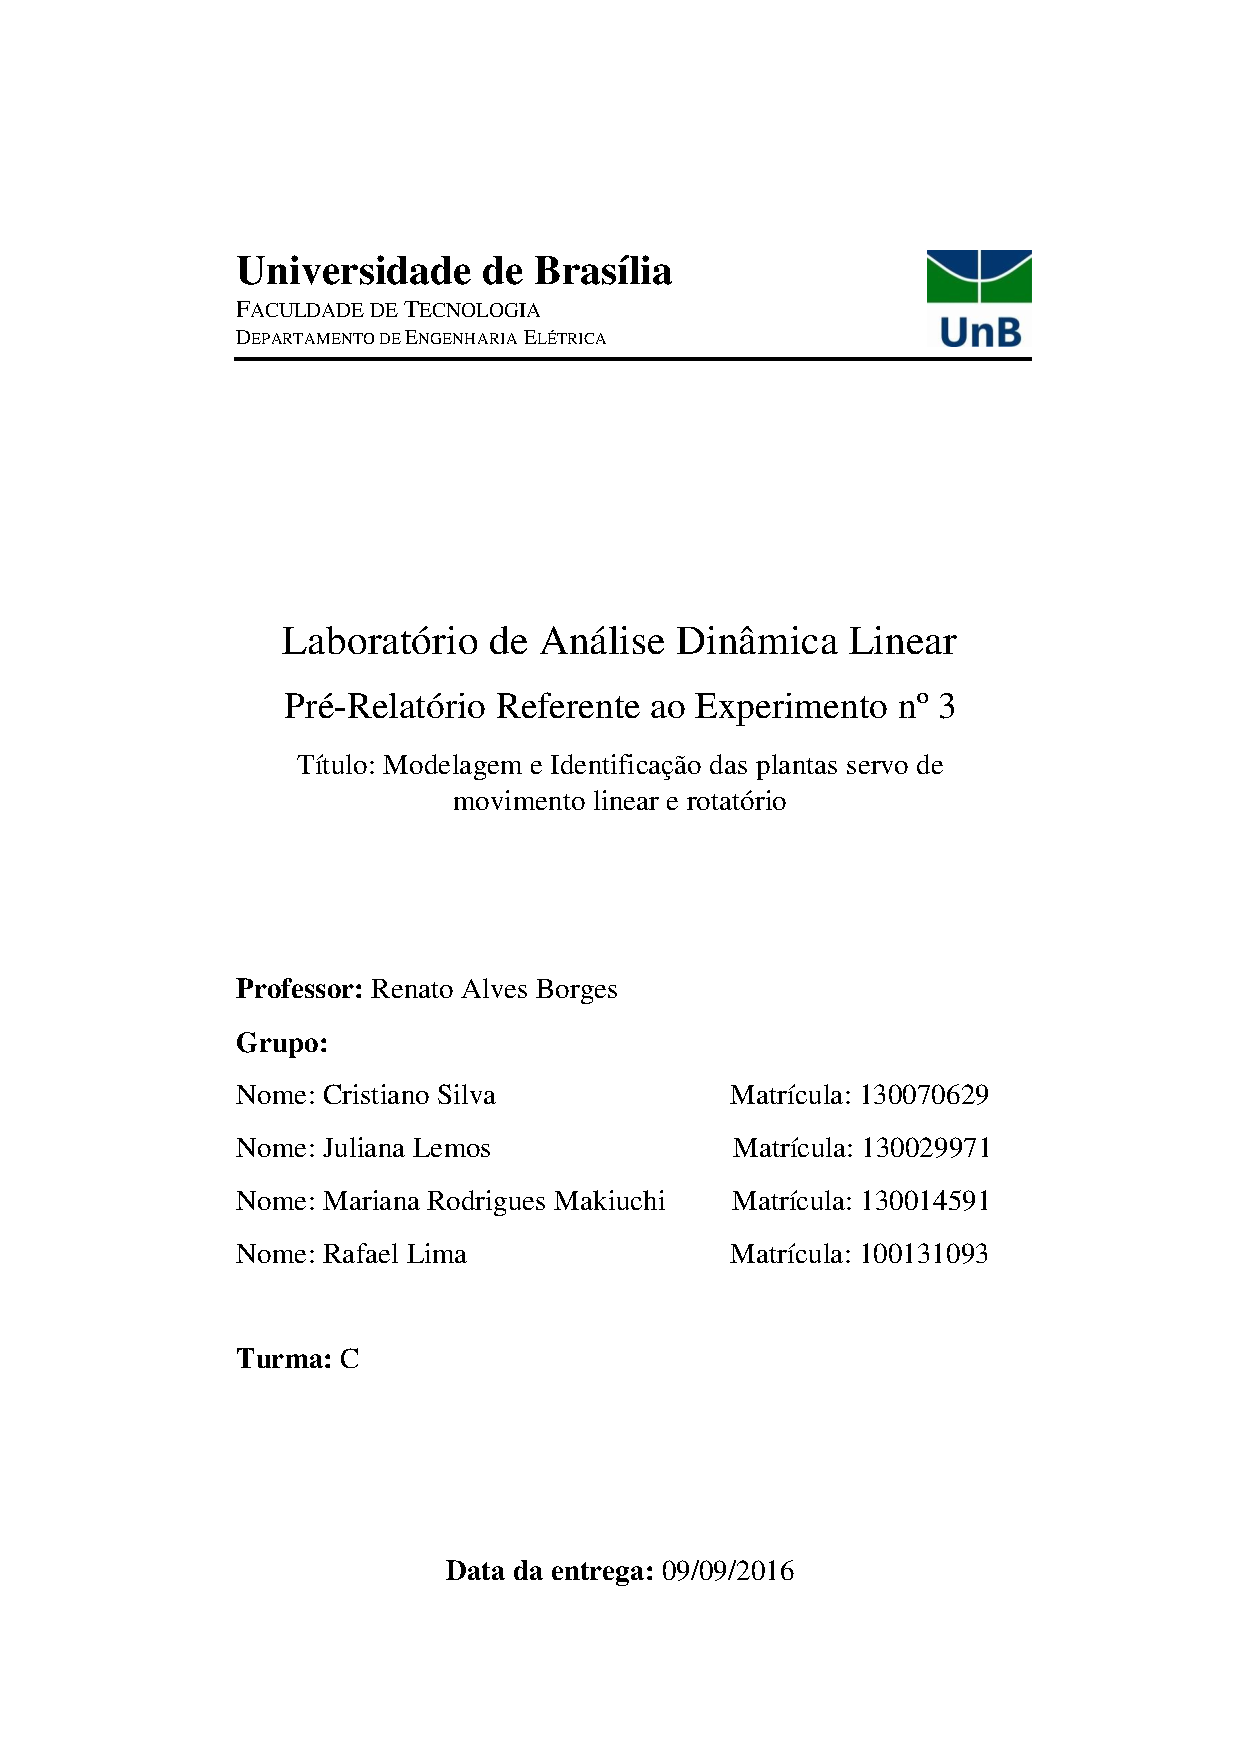
\includepdf[pages=-]{CapaPre3.pdf}
\newpage
\tableofcontents
\thispagestyle{empty}
% Conteudo -------------------------------------------------------------------
\newpage


\section{Introdução}
Introdução aqui

\section{Secção 1}
Secção aqui

\subsubsection{Código em Matlab}
Exemplo de código em Matlab

\begin{minted}[mathescape,
               linenos,
               numbersep=5pt,
               gobble=2,
               frame=lines,
               framesep=2mm]{matlab}
   % Definindo o sistema
   A = [1 1 2; 2 4 -3; 3 6 -5]
   B = [9 1 0]'
   
   % Resolvendo pelo Matlab
   X = linsolve(A,B)
   
   % Resolvendo pela regra de Crammer
   x1 = det([B A(:,2:3)])/det(A)
   x2 = det([A(:,1) B A(:,3)])/det(A)
   x3 = det([A(:,1:2) B])/det(A))
\end{minted}

\subsubsection{Resultado Obtido}
Resultados

\begin{minted}[mathescape,
               linenos,
               numbersep=5pt,
               gobble=2,
               frame=lines,
               framesep=2mm]{matlab}
    ans =
    1.0000
    2.0000
    3.0000
\end{minted}

\subsection{Exemplos de figuras}
Para o circuito elétrico definido pela Figura \ref{fig:my_label}

\begin{figure}[H]
    \centering
    \begin{circuitikz}[american voltages]
        \draw (0,1) to[L, l=$L_2$] (6,1);
        \draw (0,0) to (0,1);
        \draw (6,0) to (6,1);
        \draw (0,0) to[R,*-*, l=$R_1$] (3,0);
        \draw (3,0) to[R,*-*, l=$R_2$] (6,0);
        \draw (3,0) to[L,*-*, l_=$L_1$] (3,-3);
        \draw (6,0) to[L,*-*, l_=$L_3$ , v^=$v_L(t)$] (6,-3);
        \draw (0,-3) to (3,-3);
        \draw (3,-3) to (6,-3);
        \draw (0,-3) to[V, l=$v(t)$] (0,0);
    \end{circuitikz}
    \caption{Circuito utilizado no exercício 2 da parte 1 do experimento}
    \label{fig:my_label}
\end{figure}

%Outro exemplo de inserção de imagens via latex
%\begin{figure}[H]
%\centering
%\includegraphics[width=8cm]{./img/2b1.jpg}
%\caption{Resposta do sistema Massa Mola a um pulso de amplitude 1, largura 1}
%\label{fig:res1}
%\end{figure}

\begin{enumerate}
    \item Obtenha a função de transferência $H(s) =V_{L}(s)/V(s)$, apresentando todo o desenvolvimento da modelagem
    \item Uma vez obtida a expressão de H(s), crie uma função no Matlab que receba como parâmetros de entrada os valores das indutâncias e resistências e forneça a respectiva função de transferência (objeto função de transferência). Avalie sua função para os seguintes casos:
    \begin{enumerate}
        \item  $R_{1} = R_{2}$ = 1$\Omega$ e $L_{1} = L_{2} = L_{3}$ = 1H
        \item $R_{1}$ = 6$\Omega$, $R_{2}$ = 1$\Omega$, $L_{1}$ = 7H, $L_{2}$ = 5H e $L_{3}$ = 1H
    \end{enumerate}
\end{enumerate}

\subsubsection{Código em Matlab}

\begin{minted}[mathescape,linenos,numbersep=5pt, gobble=2,frame=lines,framesep=2mm]{matlab}
    % Declação das variáveis simbólicas
    syms L_1 L_2 L_3 R_1 R_2 V_L V S;
    syms I_1 I_2 I_3 I_4;
    
    % Representação matricial do sistema
    A(1,:) = [(R_1+L_1*S) -R_1 -L_1*S];
    A(2,:) = [-R_1 (L_2+R_2+R_1) -R_2];
    A(3,:) = [-L_1*S -(R_2) (R_2+L_3*S+L_1*S)];
    
    B(:,1) = [V 0 0]
    Xi(:,1) = [I_1 I_2 I_3]
    
    % Resolvendo pelo matlab
    X = linsolve(A,B)
    
    % Colocando S em evidência
    X = collect(X,S)
    
    % Calculando a função de transferência
    H = X(3)*L_3*S/V;
    H = collect(H,V)
    
    % Avaliando H em casos particulares
    H1 = subs(H,[L_1 L_2 L_3 R_1 R_2],[1 1 1 1 1])
    [Hn1,Hd1] = numden(H1) % Extraindo Numerador e Denominador
    
    H2 = subs(H,[L_1 L_2 L_3 R_1 R_2],[7 5 1 6 1])
    [Hn2,Hd2] = numden(H2)

    % Plotando Resultados
    TF1 = tf(double(coeffs(Hn1,S)),double(coeffs(Hd1,S)))
    figure;
    subplot(211), step(TF1)
    subplot(212), impulse(TF1)
    print('../img/adl_lab1_ex2_plot1','-dpng');
        
    TF2 = tf(double(coeffs(Hn2,S)),double(coeffs(Hd2,S)))
    figure;
    subplot(211), step(TF2)
    subplot(212), impulse(TF2)
    print('../img/adl_lab1_ex2_plot2','-dpng');
\end{minted}

\subsubsection{Tabelas}

\begin{table}[H]
    \centering
    \begin{tabular}{cccccc}
        \hline
        $H$ & $L_1$ & $L_2$ & $L_3$ & $R_1$ & $R_2$\\
        \hline
        $H_1$ & 1 & 1 & 1 & 1 & 1\\
        $H_2$ & 7 & 5 & 1 & 6 & 1\\
        \hline
    \end{tabular}
    \caption{Valores avaliados}
    \label{tab:my_label}
\end{table}

\section{Conclusão}
Conclusão aqui


\section{Bibliografia}

NISE, N.S. Control Systems Engineering. Wiley; 6ª edição. 14 de Dezembro de 2010. 944 páginas.

% ---------------------------------------------------------------------------------------
\end{document}
